\section{Évaluation des vulnérabilités du modèle de base}

Cette section présente l'évaluation de la robustesse adversariale du modèle baseline MobileNetV2 entraîné sur notre dataset. L'objectif est d'identifier les vulnérabilités du modèle face aux attaques adversariales avant l'implémentation des mécanismes de défense.

\subsection{Méthodologie d'évaluation}

L'évaluation des vulnérabilités est implémentée dans le module \texttt{attack\_baseline.py}, qui s'appuie sur une architecture de test sécurisée. Le processus d'évaluation suit une approche systématique en sandbox isolée pour garantir la reproductibilité des tests.

\paragraph{Organisation du code de test}

La structure du module d'évaluation adversariale se décompose comme suit :

\begin{verbatim}
src/experiments/baseline/
├── train_baseline.py          Entraînement du modèle baseline
├── attack_baseline.py          Tests adversariaux (FGSM)
results/adversarial_attacks/
├── fgsm_results_*.json        Résultats quantitatifs
└── security_log_*.json        Logs de sécurité
\end{verbatim}

Le testeur adversarial est encapsulé dans la classe \texttt{AdversarialTester}, qui gère le chargement sécurisé du modèle, la génération d'attaques et le logging des résultats. Cette approche modulaire permet d'isoler les tests adversariaux du reste du système et d'assurer la traçabilité complète des expérimentations via des logs immutables.

\paragraph{Configuration des tests}

Les tests sont configurés avec les paramètres suivants :

\begin{itemize}
    \item \textbf{Modèle testé} : MobileNetV2 baseline (97.5\% accuracy propre)
    \item \textbf{Dataset de test} : 204 échantillons équilibrés (102 safe, 102 dangerous)
    \item \textbf{Batch size} : 1 (tests adversariaux précis par échantillon)
    \item \textbf{Device} : CPU (reproductibilité et isolation de sécurité)
\end{itemize}

La classe \texttt{AdversarialTester} initialise le système de logging avant tout autre opération, garantissant la traçabilité complète de chaque test adversarial :

\begin{lstlisting}[language=Python, caption=Initialisation du testeur adversarial]
class AdversarialTester:
    def __init__(self, model_path, test_data_path, device='cpu'):
        self.device = torch.device(device)
        self.security_log = []
        self._log_security_event("INIT",
            "Initialisation du testeur adversarial", "INFO")

        # Chargement du modele en sandbox isolee
        self.model = self._load_model()
        self.test_loader = self._load_test_data()
\end{lstlisting}

Ce système de logging enregistre chaque événement avec un timestamp, un type d'événement et un niveau de sévérité, permettant un audit complet des tests réalisés.


\subsection{Implémentation de l'attaque FGSM}

L'attaque FGSM (Fast Gradient Sign Method) a été choisie pour cette évaluation initiale car elle représente l'attaque adversariale de référence la plus simple et rapide à calculer. L'implémentation suit la formulation classique de Goodfellow et al. : $x_{adv} = x + \epsilon \cdot \text{sign}(\nabla_x J(\theta, x, y))$, où $\epsilon$ contrôle la magnitude de la perturbation.

\paragraph{Code d'implémentation}

L'algorithme FGSM est implémenté dans la méthode \texttt{fgsm\_attack()} avec les étapes suivantes :

\begin{lstlisting}[language=Python, caption=Génération d'exemples adverses FGSM]
def fgsm_attack(self, epsilon=0.1):
    self.model.eval()

    for data, target in self.test_loader:
        data.requires_grad = True

        # Prediction propre
        output_clean = self.model(data)
        pred_clean = output_clean.argmax(dim=1)

        # Calcul du gradient
        loss = F.cross_entropy(output_clean, target)
        self.model.zero_grad()
        loss.backward()

        # Generation FGSM
        data_grad = data.grad.data
        perturbed_data = data + epsilon * data_grad.sign()
        perturbed_data = torch.clamp(perturbed_data, 0, 1)

        # Test adversarial
        output_adversarial = self.model(perturbed_data)
        pred_adversarial = output_adversarial.argmax(dim=1)
\end{lstlisting}

La perturbation est contrainte dans l'intervalle $[0,1]$ après normalisation pour garantir la validité des images adversariales. Le paramètre $\epsilon = 0.1$ a été choisi pour représenter une perturbation perceptuellement subtile mais suffisamment forte pour tester la robustesse du modèle.

\paragraph{Métriques calculées}

Pour chaque test, le système calcule quatre métriques principales stockées au format JSON :

\begin{itemize}
    \item \textbf{Clean accuracy} : Performance sur images non perturbées
    \item \textbf{Adversarial accuracy} : Performance sur images adversariales
    \item \textbf{Attack success rate} : Taux de réussite de l'attaque
    \item \textbf{Robustness degradation} : Écart entre accuracy propre et adversariale
\end{itemize}


\subsection{Résultats et identification des failles}

L'évaluation du modèle baseline révèle une vulnérabilité significative face à l'attaque FGSM. Le fichier de résultats \texttt{fgsm\_results\_20251229\_133702.json} contient les métriques suivantes :

\begin{table}[H]
    \centering
    \caption{Résultats de l'attaque FGSM sur le modèle baseline}
    \label{tab:fgsm_baseline_results}
    \begin{tabular}{lcc}
        \toprule
        \textbf{Métrique} & \textbf{Valeur} & \textbf{Interprétation} \\
        \midrule
        Échantillons testés & 204 & Ensemble de test complet \\
        Clean accuracy & 97.5\% & Excellent sur données propres \\
        Adversarial accuracy & 50.0\% & Dégradation critique \\
        Attack success rate & 50.0\% & Vulnérabilité élevée \\
        Robustness degradation & 47.5\% & Perte importante \\
        Epsilon utilisé & 0.1 & Perturbation faible \\
        \bottomrule
    \end{tabular}
\end{table}

\begin{figure}[H]
    \centering
    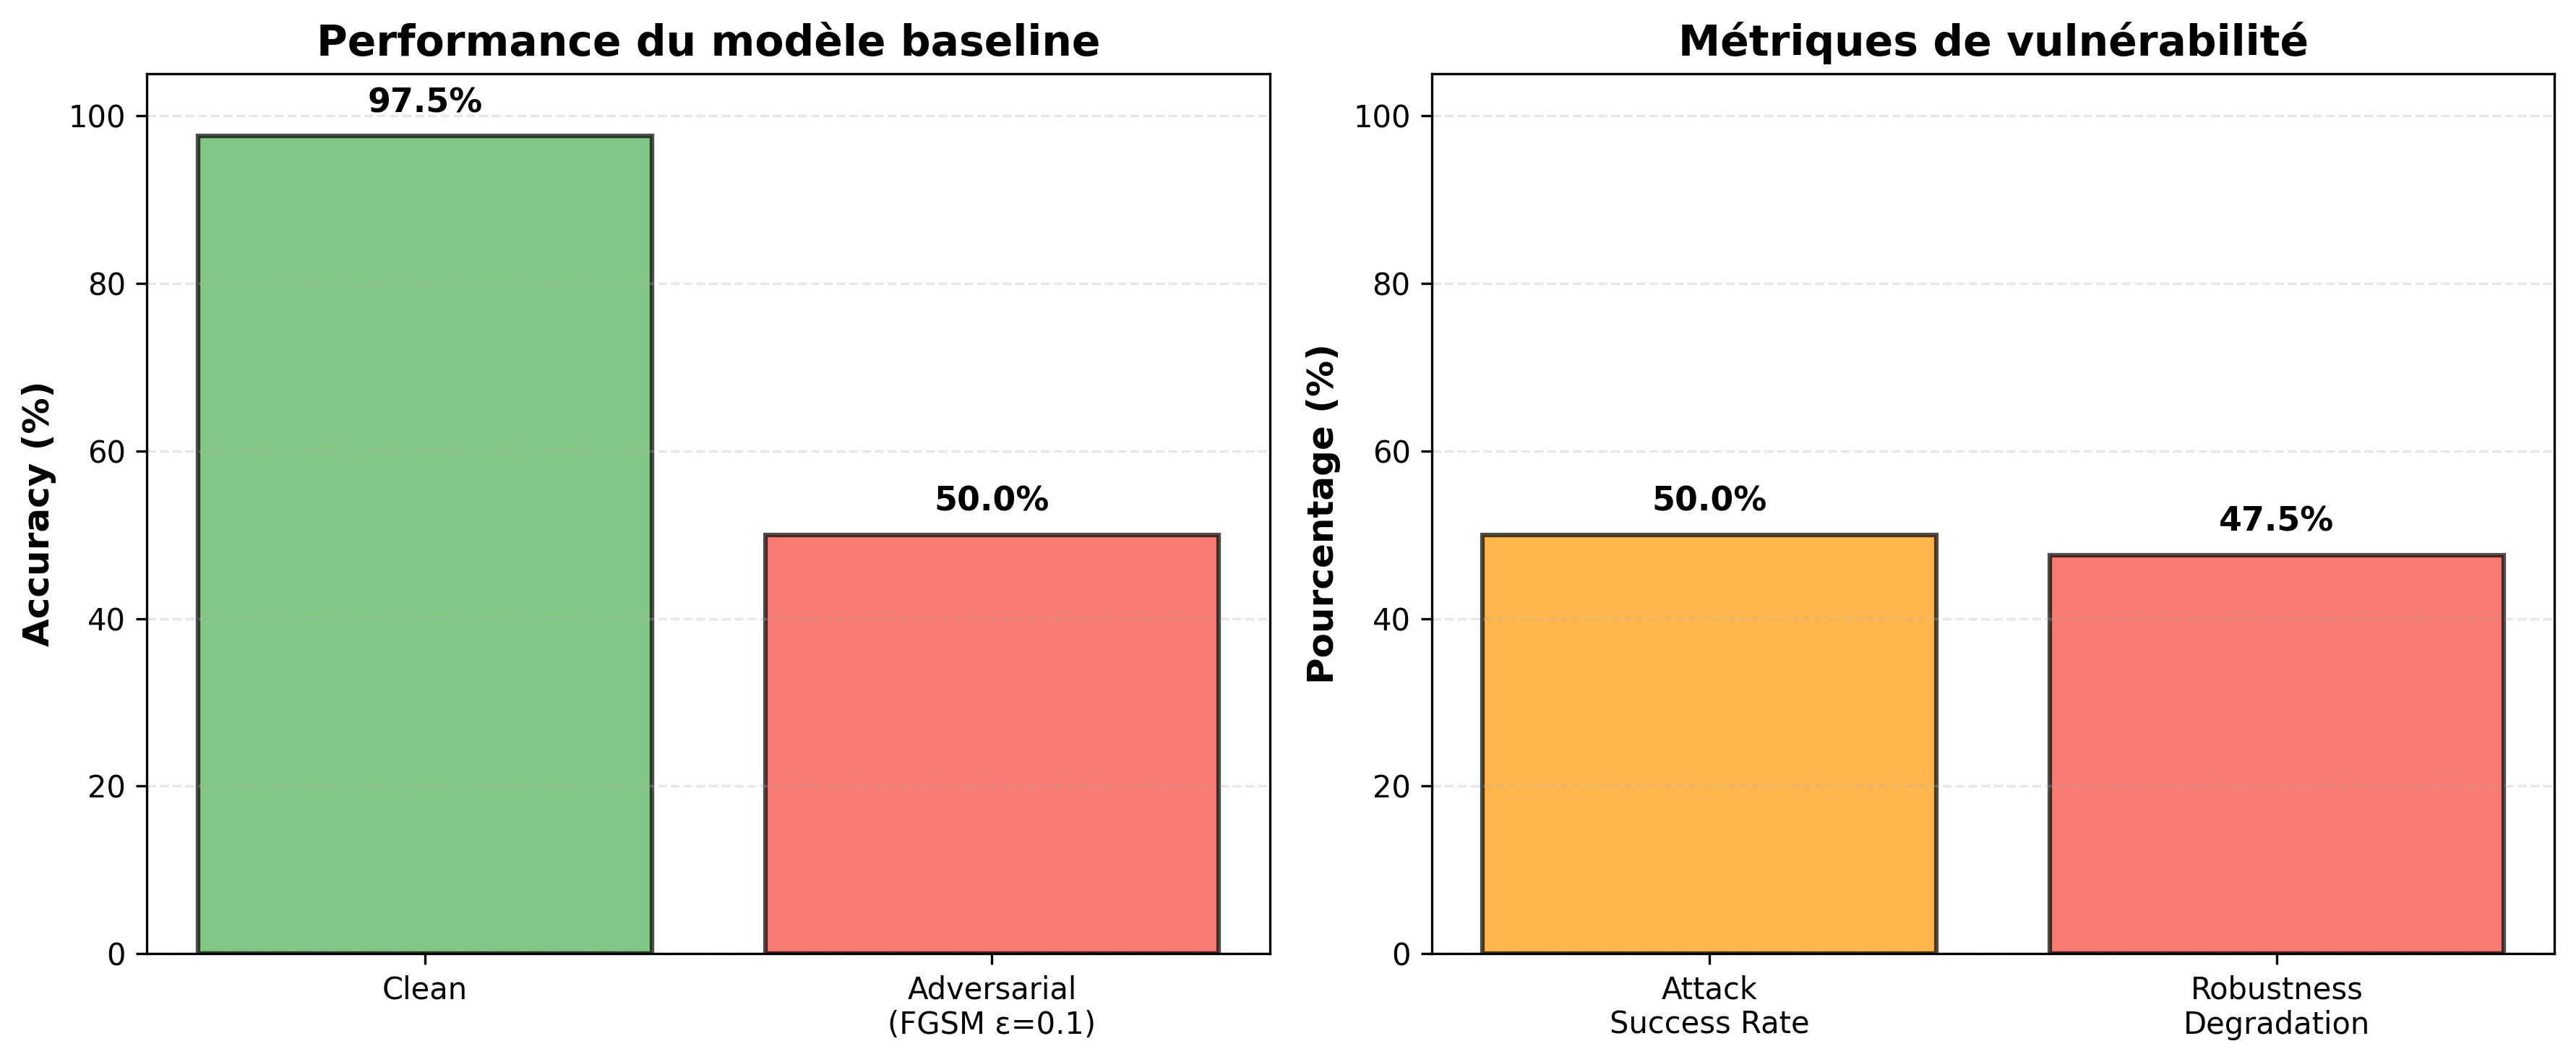
\includegraphics[width=0.9\textwidth]{figures/baseline_fgsm_comparison.png}
    \caption{Comparaison de la performance baseline : données propres vs adversariales FGSM}
    \label{fig:baseline_fgsm_comparison}
\end{figure}

\paragraph{Analyse des vulnérabilités identifiées}

Les résultats mettent en évidence trois failles majeures du modèle baseline :

\textbf{1. Sensibilité critique aux perturbations de gradient.} Avec une dégradation de 47.5\%, le modèle perd près de la moitié de sa capacité de classification face à des perturbations calculées par gradient. Cette sensibilité s'explique par l'absence de mécanismes de robustesse durant l'entraînement standard : le modèle optimise uniquement la performance sur données propres sans considération pour les variations adversariales.

\textbf{2. Vulnérabilité symétrique sur les deux classes.} L'attack success rate de 50\% indique que la vulnérabilité n'est pas limitée à une classe spécifique (safe ou dangerous), mais affecte les deux classes de manière équilibrée. Cela suggère que le modèle base ses décisions sur des features fragiles facilement manipulables par gradient descent, plutôt que sur des patterns robustes.

\textbf{3. Absence de détection d'anomalies.} Le modèle ne dispose d'aucun mécanisme pour détecter les entrées adversariales. Les exemples perturbés sont traités avec la même confiance que les images naturelles, sans alerte ni rejet. Cette lacune constitue un risque de sécurité majeur en déploiement réel, où un adversaire pourrait exploiter cette vulnérabilité pour faire passer une arme pour un objet sûr.

\paragraph{Implications pour la sécurisation}

Ces résultats justifient l'implémentation de défenses adversariales dans le pipeline d'entraînement. La section suivante (3.4) présentera le pipeline sécurisé intégrant adversarial training pour réduire significativement ces vulnérabilités. L'objectif est d'atteindre une adversarial accuracy supérieure à 80\% face à FGSM, réduisant ainsi le robustness gap à moins de 20\%.

\begin{figure}[H]
    \centering
    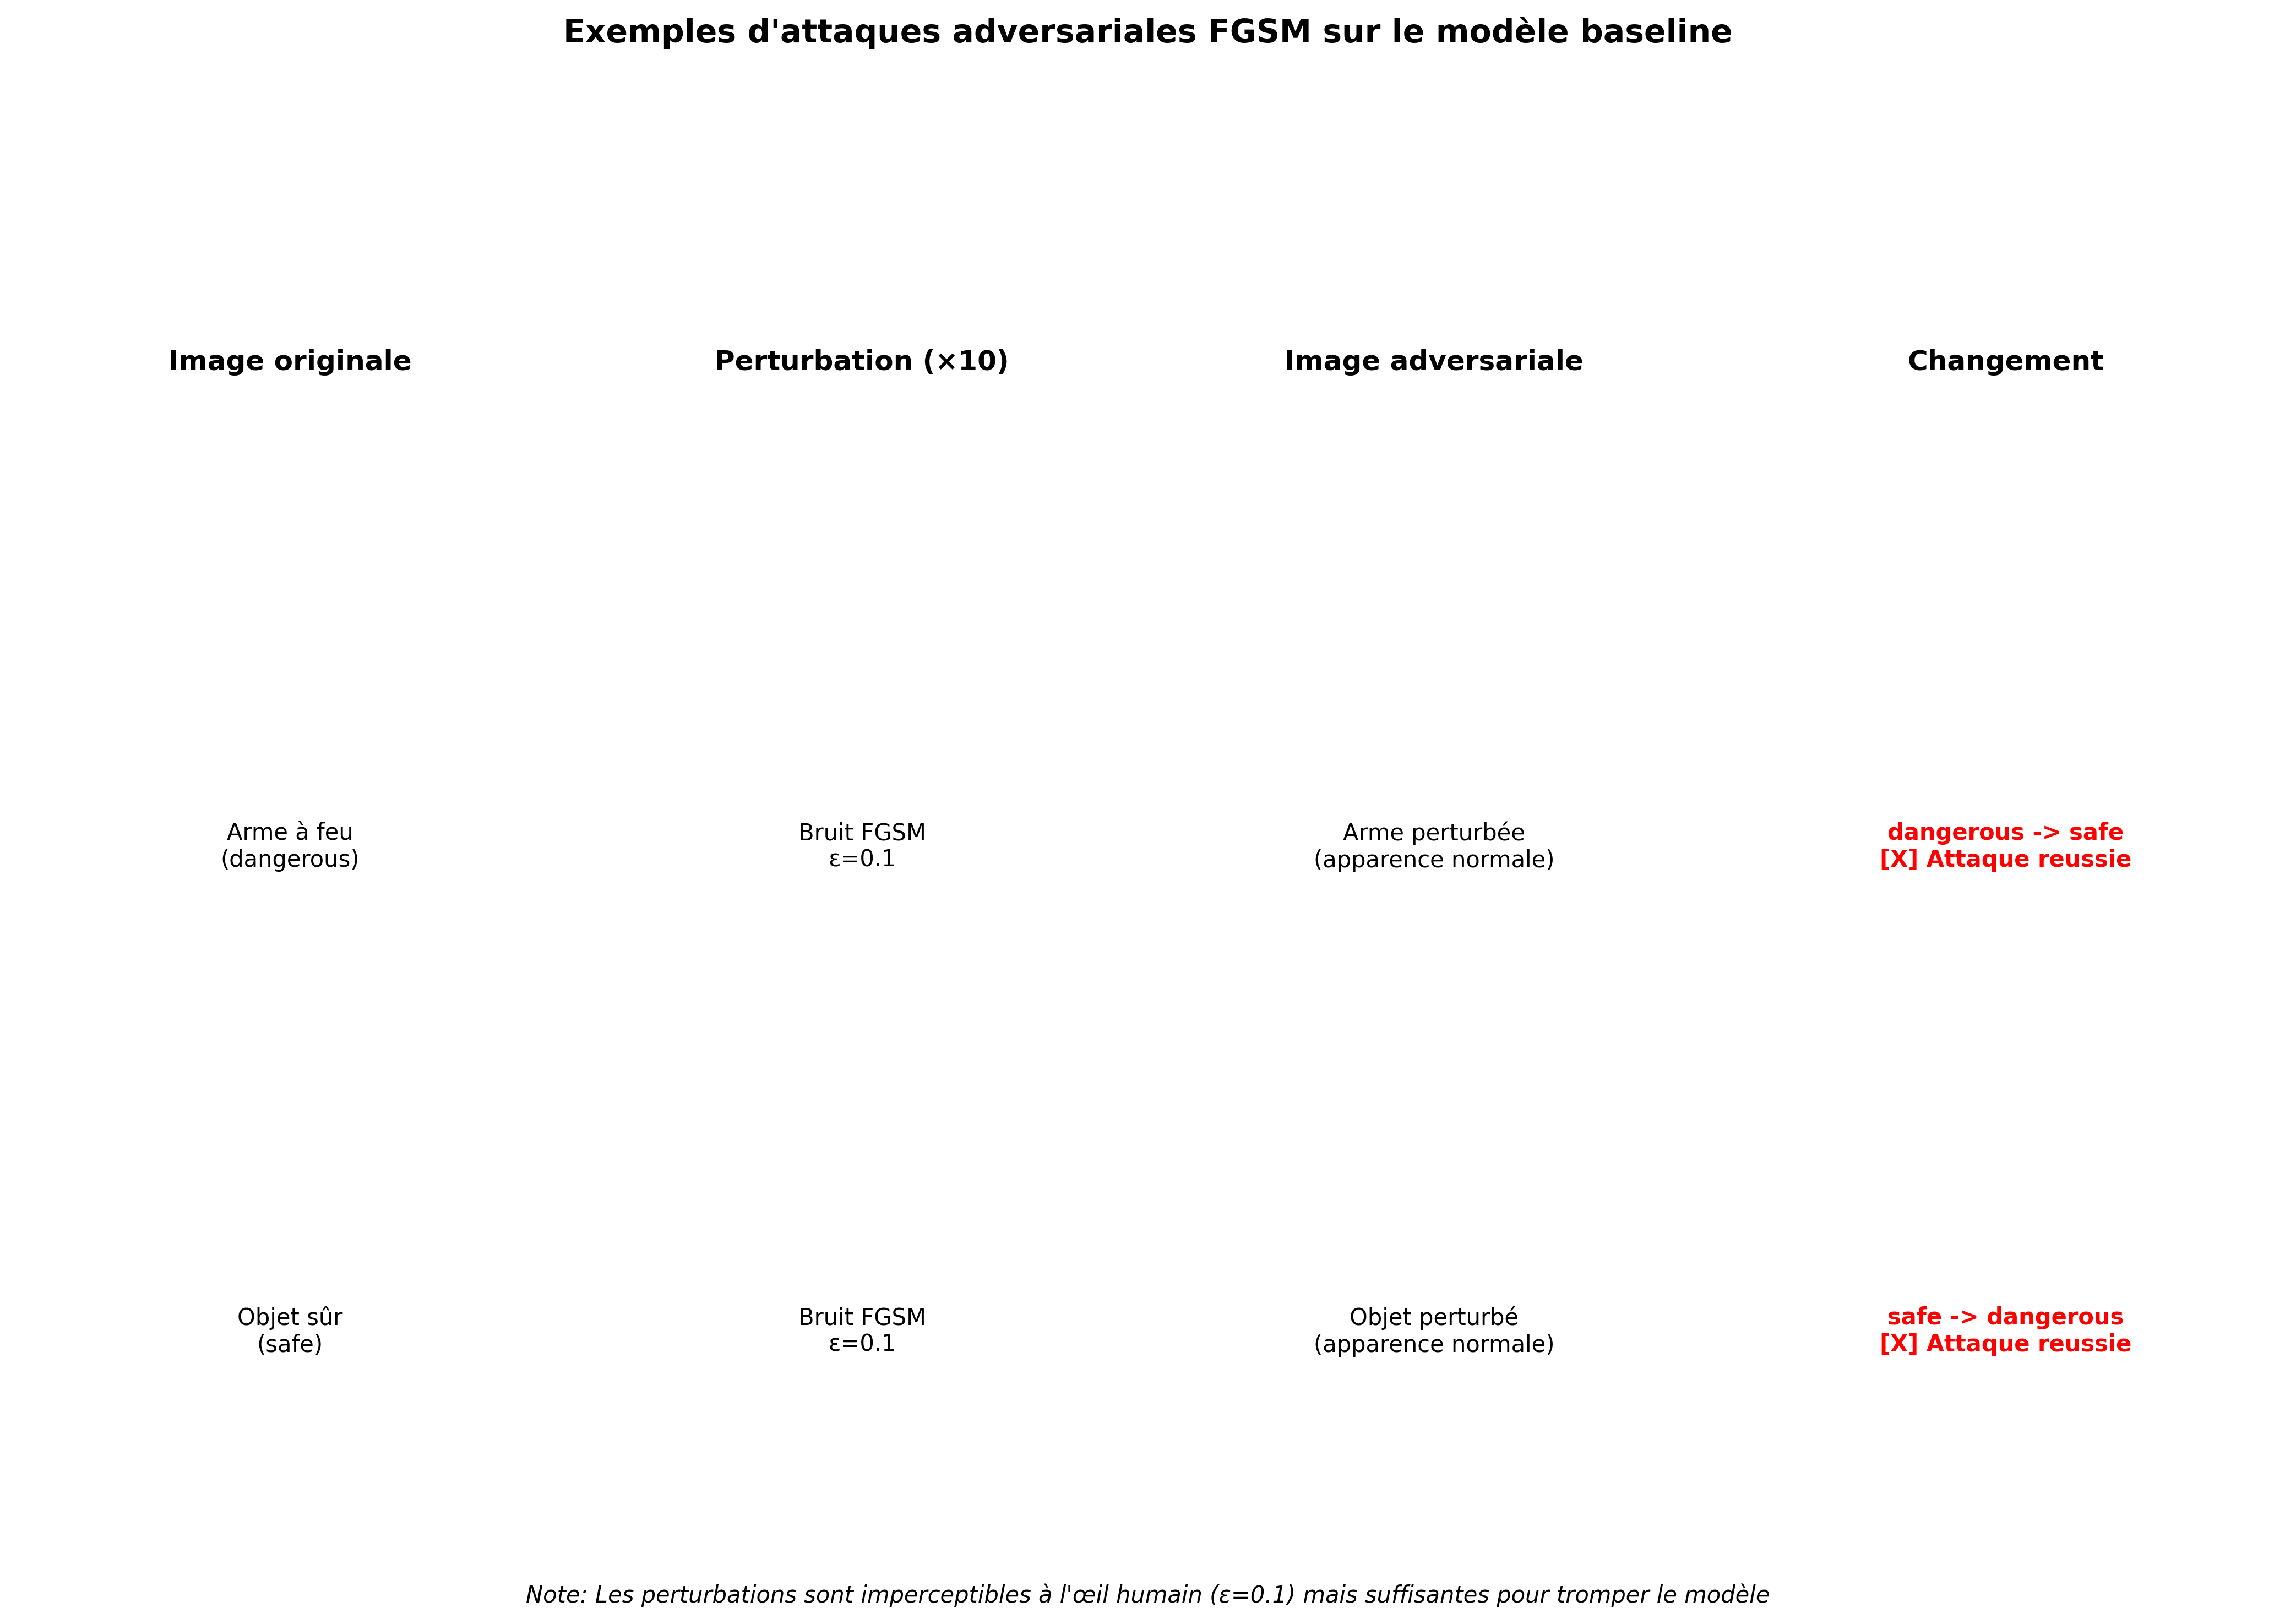
\includegraphics[width=\textwidth]{figures/fgsm_examples.png}
    \caption{Exemples d'images adversariales FGSM : originales, perturbations et prédictions}
    \label{fig:fgsm_examples}
\end{figure}